% !TEX root=../main.tex
\section{Classical Approach}
\label{sec:classical}

In an effort to better understand the vision problem presented, we first
describe a classical approach to the TurtleBot control problem. Implementation
of the methods described here was done in C++ using the OpenCV
library~\cite{opencv_library}. As described above, we seek to control the
TurtleBot robot through a track outlined with a pair of white ropes. The
commanded control of the robot must only depend on the current image from the
camera mounted on the robot.

Figure~\ref{fig:raw_img} shows an example image from the camera mounted on the
TurtleBot. As seen in this image, the lower quarter of the image is taken up by
the robot itself, effectively providing no useful information to control from.
Based on experimentation, at the constant velocity of 0.3 $m/s$ used for our
experiments, the top section of the image also does not provide any relevant
information for the current control. For these reasons, we first crop out the top
and bottom of the image to produce an image like that seen in 
Figure~\ref{fig:classical_crop}.

With the cropped image from the TurtleBot, we must first detect the ropes. As
the ropes do not change color, we depend on a simple method seg

\begin{figure}
  \centering
  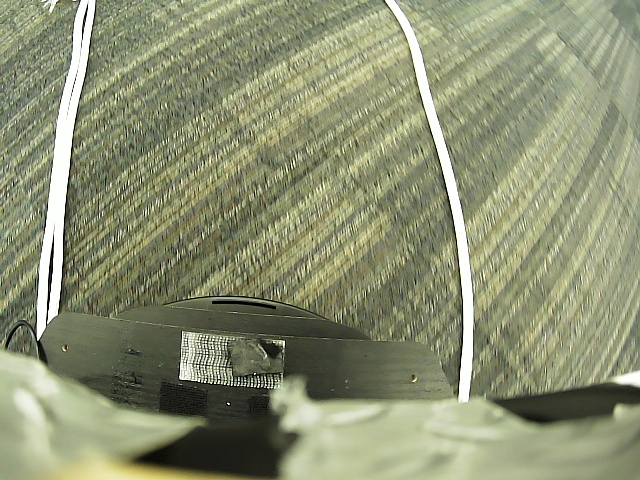
\includegraphics[scale=0.5]{figures/raw_img.png}
  \caption{Example image from the camera mounted on the TurtleBot.}
  \label{fig:raw_img}
\end{figure}

\begin{figure}
  \centering
  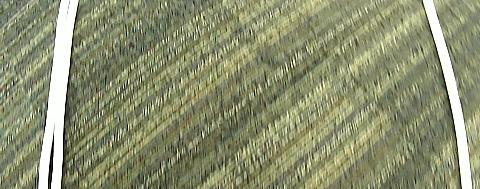
\includegraphics[scale=0.67]{figures/classical_crop.jpg}
  \caption{Cropped image from TurtleBot.}
  \label{fig:classical_crop}
\end{figure}

\begin{figure}
  \centering
  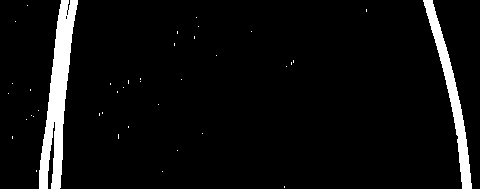
\includegraphics[scale=0.5]{figures/classical_thresh.jpg}
  \caption{TurtleBot image after thresholding.}
  \label{fig:classical_thresh}
\end{figure}

\begin{figure}
  \centering
  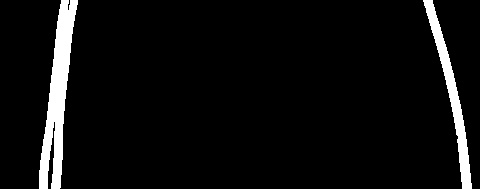
\includegraphics[scale=0.5]{figures/classical_contours.jpg}
  \caption{TurtleBot image with only largest contours.}
  \label{fig:classical_contours}
\end{figure}

\begin{figure}
  \centering
  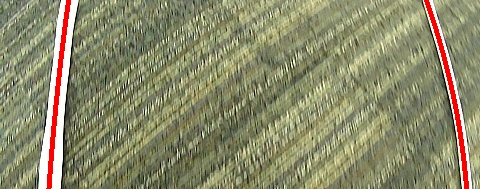
\includegraphics[scale=0.5]{figures/classical_fit.jpg}
  \caption{TurtleBot image with splines fit to largest contours.}
  \label{fig:classical_fit}
\end{figure}

\begin{figure}
  \centering
  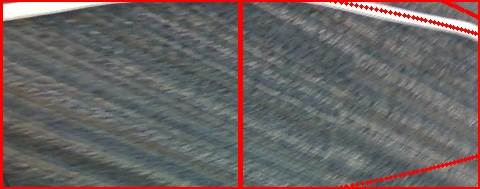
\includegraphics[scale=0.5]{figures/classical_fail.jpg}
  \caption{Example of a failure mode of the classical end-to-end control method.}
  \label{fig:classical_fail}
\end{figure}
